
\begin{figure} \centering 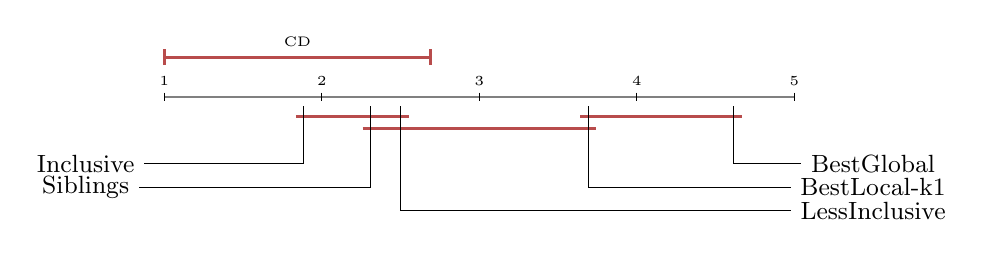
\begin{tikzpicture}[xscale=2]
\node (Label) at  (01.8450,0.7) {\tiny{CD}}; % the label
\draw[very thick, color = red!60!black!70](01.0000, 0.5) -- (02.6900, 0.5);
\foreach \x in {01.0000,02.6900} \draw[thick,color = red!60!black!70] (\x, 0.4) -- (\x, 0.6);

\draw[gray, thick](01.0000, 0) -- (05.0000, 0);
\foreach \x in {01.0000,02.0000,03.0000,04.0000,05.0000}\draw (\x cm,1.5pt) -- (\x cm, -1.5pt);
\node (Label) at (01.0000,0.2) {\tiny{1}};
\node (Label) at (02.0000,0.2) {\tiny{2}};
\node (Label) at (03.0000,0.2) {\tiny{3}};
\node (Label) at (04.0000,0.2) {\tiny{4}};
\node (Label) at (05.0000,0.2) {\tiny{5}};
\draw[very thick, color = red!60!black!70](01.8350,-00.2500) -- ( 02.5500,-00.2500);
\draw[very thick, color = red!60!black!70](02.2580,-00.4000) -- ( 03.7420,-00.4000);
\draw[very thick, color = red!60!black!70](03.6420,-00.2500) -- ( 04.6650,-00.2500);
\node (Point) at (01.8850, 0){};  \node (Label) at (0.5,-00.8500){\small{Inclusive}}; \draw (Point) |- (Label);
\node (Point) at (02.3080, 0){};  \node (Label) at (0.5,-01.1500){\small{Siblings}}; \draw (Point) |- (Label);
\node (Point) at (04.6150, 0){};  \node (Label) at (5.5,-00.8500){\small{BestGlobal}}; \draw (Point) |- (Label);
\node (Point) at (03.6920, 0){};  \node (Label) at (5.5,-01.1500){\small{BestLocal-k1}}; \draw (Point) |- (Label);
\node (Point) at (02.5000, 0){};  \node (Label) at (5.5,-01.4500){\small{LessInclusive}}; \draw (Point) |- (Label);
\end{tikzpicture}
\caption{./f1micro-nb-mln.property}
\label{fig:}
\end{figure}

